%-----------------------------------------------------------------------------------------------------------------------------------------------%
%	The MIT License (MIT)
%
%	Copyright (c) 2019 Jan Küster
%
%	Permission is hereby granted, free of charge, to any person obtaining a copy
%	of this software and associated documentation files (the "Software"), to deal
%	in the Software without restriction, including without limitation the rights
%	to use, copy, modify, merge, publish, distribute, sublicense, and/or sell
%	copies of the Software, and to permit persons to whom the Software is
%	furnished to do so, subject to the following conditions:
%	
%	THE SOFTWARE IS PROVIDED "AS IS", WITHOUT WARRANTY OF ANY KIND, EXPRESS OR
%	IMPLIED, INCLUDING BUT NOT LIMITED TO THE WARRANTIES OF MERCHANTABILITY,
%	FITNESS FOR A PARTICULAR PURPOSE AND NONINFRINGEMENT. IN NO EVENT SHALL THE
%	AUTHORS OR COPYRIGHT HOLDERS BE LIABLE FOR ANY CLAIM, DAMAGES OR OTHER
%	LIABILITY, WHETHER IN AN ACTION OF CONTRACT, TORT OR OTHERWISE, ARISING FROM,
%	OUT OF OR IN CONNECTION WITH THE SOFTWARE OR THE USE OR OTHER DEALINGS IN
%	THE SOFTWARE.
%	
%
%-----------------------------------------------------------------------------------------------------------------------------------------------%


%============================================================================%
%
%	DOCUMENT DEFINITION
%
%============================================================================%

%we use article class because we want to fully customize the page and don't use a cv template
\documentclass[10pt,A4]{article}	


%----------------------------------------------------------------------------------------
%	ENCODING
%----------------------------------------------------------------------------------------

% we use utf8 since we want to build from any machine
\usepackage[utf8]{inputenc}		

%----------------------------------------------------------------------------------------
%	LOGIC
%----------------------------------------------------------------------------------------

% provides \isempty test
\usepackage{xstring, xifthen}

%----------------------------------------------------------------------------------------
%	FONT BASICS
%----------------------------------------------------------------------------------------

% some tex-live fonts - choose your own

%\usepackage[defaultsans]{droidsans}
%\usepackage[default]{comfortaa}
%\usepackage{cmbright}
\usepackage[default]{raleway}
%\usepackage{fetamont}
%\usepackage[default]{gillius}
%\usepackage[light,math]{iwona}
%\usepackage[thin]{roboto} 
\usepackage{fontawesome}

% set font default
\renewcommand*\familydefault{\sfdefault} 	
\usepackage[T1]{fontenc}

% more font size definitions
\usepackage{moresize}

%----------------------------------------------------------------------------------------
%	FONT AWESOME ICONS
%---------------------------------------------------------------------------------------- 

% include the fontawesome icon set
\usepackage{fontawesome}

% use to vertically center content
% credits to: http://tex.stackexchange.com/questions/7219/how-to-vertically-center-two-images-next-to-each-other
\newcommand{\vcenteredinclude}[1]{\begingroup
\setbox0=\hbox{\includegraphics{#1}}%
\parbox{\wd0}{\box0}\endgroup}

% use to vertically center content
% credits to: http://tex.stackexchange.com/questions/7219/how-to-vertically-center-two-images-next-to-each-other
\newcommand*{\vcenteredhbox}[1]{\begingroup
\setbox0=\hbox{#1}\parbox{\wd0}{\box0}\endgroup}

% icon shortcut
\newcommand{\icon}[3] { 							
	\makebox(#2, #2){\textcolor{maincol}{\csname fa#1\endcsname}}
}	

% icon with text shortcut
\newcommand{\icontext}[4]{ 						
	\vcenteredhbox{\icon{#1}{#2}{#3}}  \hspace{2pt}  \parbox{0.9\mpwidth}{\textcolor{#4}{#3}}
}

% icon with website url
\newcommand{\iconhref}[5]{ 						
    \vcenteredhbox{\icon{#1}{#2}{#5}}  \hspace{2pt} \href{#4}{\textcolor{#5}{#3}}
}

% icon with email link
\newcommand{\iconemail}[5]{ 						
    \vcenteredhbox{\icon{#1}{#2}{#5}}  \hspace{2pt} \href{mailto:#4}{\textcolor{#5}{#3}}
}

%----------------------------------------------------------------------------------------
%	PAGE LAYOUT  DEFINITIONS
%----------------------------------------------------------------------------------------

% page outer frames (debug-only)
% \usepackage{showframe}		

% we use paracol to display breakable two columns
\usepackage{paracol}

% define page styles using geometry
\usepackage[a4paper]{geometry}

% remove all possible margins
\geometry{top=1cm, bottom=1cm, left=1cm, right=1cm}

\usepackage{fancyhdr}
\pagestyle{empty}

% space between header and content
% \setlength{\headheight}{0pt}

% indentation is zero
\setlength{\parindent}{0mm}

%----------------------------------------------------------------------------------------
%	TABLE /ARRAY DEFINITIONS
%---------------------------------------------------------------------------------------- 

% extended aligning of tabular cells
\usepackage{array}

% custom column right-align with fixed width
% use like p{size} but via x{size}
\newcolumntype{x}[1]{%
>{\raggedleft\hspace{0pt}}p{#1}}%


%----------------------------------------------------------------------------------------
%	GRAPHICS DEFINITIONS
%---------------------------------------------------------------------------------------- 

%for header image
\usepackage{graphicx}

% use this for floating figures
% \usepackage{wrapfig}
% \usepackage{float}
% \floatstyle{boxed} 
% \restylefloat{figure}

%for drawing graphics		
\usepackage{tikz}				
\usetikzlibrary{shapes, backgrounds,mindmap, trees}

%----------------------------------------------------------------------------------------
%	Color DEFINITIONS
%---------------------------------------------------------------------------------------- 
\usepackage{transparent}
\usepackage{color}

% primary color
\definecolor{maincol}{RGB}{ 30, 144, 255 }

% accent color, secondary
% \definecolor{accentcol}{RGB}{ 250, 150, 10 }

% dark color
\definecolor{darkcol}{RGB}{ 70, 70, 70 }

% light color
\definecolor{lightcol}{RGB}{245,245,245}


% Package for links, must be the last package used
\usepackage[hidelinks]{hyperref}

% returns minipage width minus two times \fboxsep
% to keep padding included in width calculations
% can also be used for other boxes / environments
\newcommand{\mpwidth}{\linewidth-\fboxsep-\fboxsep}
	


%============================================================================%
%
%	CV COMMANDS
%
%============================================================================%

%----------------------------------------------------------------------------------------
%	 CV LIST
%----------------------------------------------------------------------------------------

% renders a standard latex list but abstracts away the environment definition (begin/end)
\newcommand{\cvlist}[1] {
	\begin{itemize}{#1}\end{itemize}
}

%----------------------------------------------------------------------------------------
%	 CV TEXT
%----------------------------------------------------------------------------------------

% base class to wrap any text based stuff here. Renders like a paragraph.
% Allows complex commands to be passed, too.
% param 1: *any
\newcommand{\cvtext}[1] {
	\begin{tabular*}{1\mpwidth}{p{0.98\mpwidth}}
		\parbox{1\mpwidth}{#1}
	\end{tabular*}
}

%----------------------------------------------------------------------------------------
%	CV SECTION
%----------------------------------------------------------------------------------------

% Renders a a CV section headline with a nice underline in main color.
% param 1: section title
\newcommand{\cvsection}[1] {
	\vspace{14pt}
	\cvtext{
		\textbf{\LARGE{\textcolor{darkcol}{\uppercase{#1}}}}\\[-4pt]
		\textcolor{maincol}{ \rule{0.1\textwidth}{2pt} } \\
	}
}

%----------------------------------------------------------------------------------------
%	META SKILL
%----------------------------------------------------------------------------------------

% Renders a progress-bar to indicate a certain skill in percent.
% param 1: name of the skill / tech / etc.
% param 2: level (for example in years)
% param 3: percent, values range from 0 to 1
\newcommand{\cvskill}[3] {
	\begin{tabular*}{1\mpwidth}{p{0.72\mpwidth}  r}
 		\textcolor{black}{\textbf{#1}} & \textcolor{maincol}{\textbf{#2}}\\
	\end{tabular*}%
	
	\hspace{4pt}
	\begin{tikzpicture}[scale=1,rounded corners=2pt,very thin]
		\fill [lightcol] (0,0) rectangle (1\mpwidth, 0.15);
		\fill [maincol] (0,0) rectangle (#3\mpwidth, 0.15);
  	\end{tikzpicture}%
}


%----------------------------------------------------------------------------------------
%	 CV EVENT
%----------------------------------------------------------------------------------------

% Renders a table and a paragraph (cvtext) wrapped in a parbox (to ensure minimum content
% is glued together when a pagebreak appears).
% Additional Information can be passed in text or list form (or other environments).
% the work you did
% param 1: time-frame i.e. Sep 14 - Jan 15 etc.
% param 2:	 event name (job position etc.)
% param 3: Customer, Employer, Industry
% param 4: Short description
% param 5: work done (optional)
% param 6: technologies include (optional)
% param 7: achievements (optional)
\newcommand{\cvevent}[7] {
	
	% we wrap this part in a parbox, so title and description are not separated on a pagebreak
	% if you need more control on page breaks, remove the parbox
	\parbox{\mpwidth}{
		\begin{tabular*}{1\mpwidth}{p{0.72\mpwidth}  r}
	 		\textcolor{black}{\textbf{#2}} & \colorbox{maincol}{\makebox[0.33\mpwidth]{\textcolor{white}{#1}}} \\
			\textcolor{maincol}{\textbf{#3}} & \\
		\end{tabular*}\\[8pt]
	
		\ifthenelse{\isempty{#4}}{}{
			\cvtext{#4}\\
		}
	}

	\ifthenelse{\isempty{#5}}{}{
		\vspace{9pt}
		{#5}
	}

	\ifthenelse{\isempty{#6}}{}{
		\vspace{9pt}
		\cvtext{\textbf{Technologies include:}}\\
		{#6}
	}

	\ifthenelse{\isempty{#7}}{}{
		\vspace{9pt}
		\cvtext{\textbf{Achievements include:}}\\
		{#7}
	}
	\vspace{14pt}
}

%----------------------------------------------------------------------------------------
%	 CV META EVENT
%----------------------------------------------------------------------------------------

% Renders a CV event on the sidebar
% param 1: title
% param 2: subtitle (optional)
% param 3: customer, employer, etc,. (optional)
% param 4: info text (optional)
\newcommand{\cvmetaevent}[4] {
	\textcolor{maincol} {\cvtext{\textbf{\begin{flushleft}#1\end{flushleft}}}}

	\ifthenelse{\isempty{#2}}{}{
	\textcolor{darkcol} {\cvtext{\textbf{#2}} }
	}

	\ifthenelse{\isempty{#3}}{}{
		\cvtext{{ \textcolor{black} {#3} }}\\
	}

	\cvtext{#4}\\[14pt]
}

%---------------------------------------------------------------------------------------
%	QR CODE
%----------------------------------------------------------------------------------------

% Renders a qrcode image (centered, relative to the parentwidth)
% param 1: percent width, from 0 to 1
\newcommand{\cvqrcode}[1] {
	\begin{center}
		\includegraphics[width={#1}\mpwidth]{qrcode}
	\end{center}
}


%============================================================================%
%
%
%
%	DOCUMENT CONTENT
%
%
%
%============================================================================%
\begin{document}
\columnratio{0.35}
\setlength{\columnsep}{2.2em}
\setlength{\columnseprule}{4pt}
\colseprulecolor{lightcol}
\begin{paracol}{2}
\begin{leftcolumn}
%---------------------------------------------------------------------------------------
%	META IMAGE
%----------------------------------------------------------------------------------------
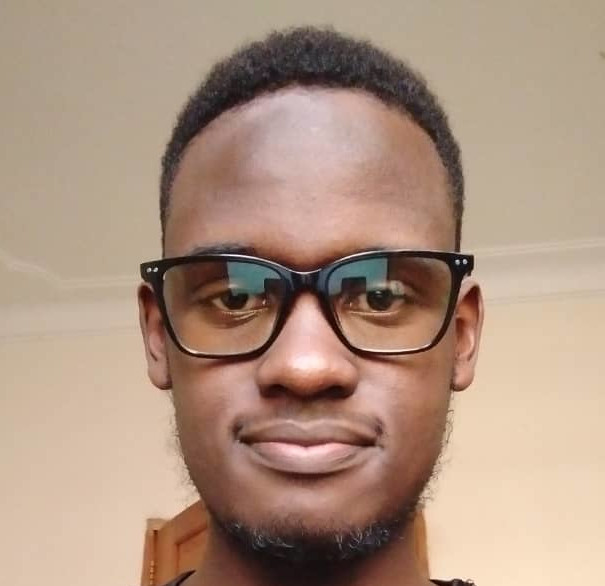
\includegraphics[width=\linewidth]{profile.jpeg}	%trimming relative to image size


%-------------------------------------------------------------------------------------
% PERSONAL DATA
% ------------------------------------------------------------------------------------

\cvsection{PERSONAL DATA}
\textbf{ \textcolor{blue}{ Nationality}}\\
\textbf{ Ugandan }
\\
\\
\textbf{ \textcolor{blue}{Gender}}\\
\textbf{ Male }

\vfull\null


%-------------------------------------------------------------------------------------
% CONTACT INFOMATION
% ------------------------------------------------------------------------------------

\cvsection{CONTACT}
	
\icontext{MapMarker}{12}{Uganda/Kampala/Bukoto}{black}\\[6pt]
\icontext{MobilePhone}{12}{+25677431 5917}{black}\\[6pt]
\iconemail{Envelope}{12}{kabbajosephtimothy@gmail.com}{kabbajosephtimothy@gmail.com}{black}\\[6pt]
\icontext{\faLinkedin}{12}{https://linkedin.com/in/kabba-joseph-timothy}{black}\\[6pt]
\icontext{\faGithub}{12}{https://github.com/josephkabba}{black}\\[6pt]

%---------------------------------------------------------------------------------------
%	META SKILLS
%----------------------------------------------------------------------------------------
\cvsection{SKILLS}

\cvskill{Python} {5+ yrs} {1} \\[-2pt]

\cvskill{Android} {6+ yrs} {1} \\[-2pt]

\cvskill{Android Studio} {6+ yrs} {1} \\[-2pt]

\cvskill{Kotlin} {4+ yrs} {1} \\[-2pt]

\cvskill{Java} {6+ yrs} {1} \\[-2pt]

\cvskill{SQL} {4+ yrs} {1} \\[-2pt]

\cvskill{Open Source Tools} {5+ yrs} {1} \\[-2pt]

\cvskill{Typescript} {3+ yrs} {0.90} \\[-2pt]

\cvskill{Dart} {2+ yrs} {0.90} \\[-2pt]

\cvskill{Javascript} {4+ yrs} {0.90} \\[-2pt]

\cvskill{Html/CSS} {6+ yrs} {0.72} \\[-2pt]

\cvskill{Mongo DB} {2+ yrs} {0.60} \\[-2pt]

\cvskill{Bash Script} {2+ yrs} {0.50} \\[-2pt]

\cvskill{Django} {1+ yrs} {0.40} \\[-2pt]

\cvskill{Solidity} {3+ yrs} {0.30} \\[-2pt]

\vfill\null


% ---------------------------------------------------------------------------
% SOFTWARE
% ---------------------------------------------------------------------------

\cvsection{SOFTWARE}

\cvskill{VS Code} {5+ yrs} {1} \\[-2pt]

\cvskill{Android Studio} {6+ yrs} {1} \\[-2pt]

\cvskill{Intellij} {6+ yrs} {1} \\[-2pt]

\cvskill{MS Word} {10+ yrs} {1} \\[-2pt]

\cvskill{MS Excel} {10+ yrs} {1} \\[-2pt]

\cvskill{Git} {6+ yrs} {1} \\[-2pt]

\cvskill{Terminal} {2+ yrs} {0.90} \\[-2pt]

\cvskill{Firebase} {4+ yrs} {0.90} \\[-2pt]

\cvskill{Linux} {3+ yrs} {0.60} \\[-2pt]

\cvskill{Figma} {2+ yrs} {0.50} \\[-2pt]

\cvskill{Google Cloud platform} {3+ yrs} {0.40} \\[-2pt]

\cvskill{Gimp} {3+ yrs} {0.20} \\[-2pt]



\vfill\null

\cvsection{LANGUAGES}

\cvskill{English} {Excellent} {1} \\[-2pt]

\cvskill{Luganda} {Good} {0.80} \\[-2pt]

\cvskill{Kiswahili} {Basic} {0.20} \\[-2pt]

\cvskill{French} {Basic} {0.20} \\[-2pt]


%---------------------------------------------------------------------------------------
%	EDUCATION
%----------------------------------------------------------------------------------------
\vfill\null
\vfill
\cvsection{EDUCATION}

\cvmetaevent
{AUG 2019 - AUG 2022}
{Bachelor of Science in Computer Science}
{MAKERERE UNIVERSITY}
{Computer Science}

\cvmetaevent
{2017 - 2018}
{Uganda Advanced Certificate of Education (UACE)}
{SEETA HIGH SCHOOL}
{Physics, Mathematics and Geometry Drawing (PTM), ICT, GP}

\cvmetaevent
{2013 - 2016}
{Uganda Certificate of Education (UCE)}
{SEETA HIGH SCHOOL}
{}

\cvmetaevent
{2006 - 2012}
{Primary Leaving Examination (PLE)}
{LOHANA SCHOOLS (KOLOLO)}
{}

\vfill\null

%---------------------------------------------------------------------------------------
%	INTERESTS
%----------------------------------------------------------------------------------------
\cvsection{INTERESTS}
\cvlist{
		\item Computer programming
		\item Gyming
		\item Basket ball
		\item Web3 and blockchain 
		\item Building relationships with people
	}
	
\vfill\null

%---------------------------------------------------------------------------------------
%	REFERENCES
%----------------------------------------------------------------------------------------
\cvsection{REFERENCES}

\textbf{ Mr Peter Simon Kabba}\\[6pt]
\icontext{MobilePhone}{12}{+256755556464}{black}\\[6pt]
\iconemail{Envelope}{12}{pskabba@gmail.com}{black}\\[6pt]
\\
\\

\textbf{ Mr Peter Simon Ojok}\\[6pt]
\icontext{MobilePhone}{12}{+256772241709}{black}\\[6pt]
\iconemail{Envelope}{12}{simonpojok@gmail.com}{black}\\[6pt]
\\
\\

\textbf{ Mr Fredrick Kasoma}\\[6pt]
\icontext{MobilePhone}{12}{+256700408387}{black}\\[6pt]
\iconemail{Envelope}{12}{kfredrick35@gmail.com}{black}\\[6pt]






\mbox{} % hotfix to place qrcode on the bottom when there are not other elements
\vfill

\end{leftcolumn}
\begin{rightcolumn}
%---------------------------------------------------------------------------------------
%	TITLE  HEADER
%----------------------------------------------------------------------------------------
\fcolorbox{white}{darkcol}{\begin{minipage}[c][3.5cm][c]{1\mpwidth}
	\begin {center}
		\HUGE{ \textbf{ \textcolor{white}{ \uppercase{ KABBA JOSEPH TIMOTHY } } } } \\[-24pt]
		\textcolor{white}{ \rule{0.1\textwidth}{1.25pt} } \\[4pt]
		\large{ \textcolor{white} {Software Engineer (Mobile and Fullstack)} }
	\end {center}
\end{minipage}} \\[14pt]
\vspace{-12pt}

%---------------------------------------------------------------------------------------
%	PROFILE
%----------------------------------------------------------------------------------------
\vfill\null
\cvsection{PROFILE}

\cvtext{I am a software developer with 5 years of professional experience and 7 years of overall experience in developing modern android mobile applications with android development tools such as Kotlin, Java, Android Studio, Jetpack Libraries, jetpack compose, MVVM and Clean Architecture. \\

I am also experienced in developing React.js applications and back-end applications using Typescript, Mongo Database, Redis and Node.js. My strongest skill is mobile development. I love learning new technologies and improving my soft and technical skills. Also have a firm foundation in math skills and logical thinking.\\

Have experience working in startups and fast-moving teams with fixed deadlines. Very flexible with learning different technologies, am also able to adapt. I am a complex problem-solver with analytical and driven mindset. Dedicated to achieving demanding development objectives according to tight schedules while producing impeccable code.\\

}

%---------------------------------------------------------------------------------------
%	WORK EXPERIENCE
%----------------------------------------------------------------------------------------
\vfill\null
\cvsection{WORK EXPERIENCE}

\cvevent
	{AUG 2021 - JULY 2022}
	{Lead Android Engineer and Backend Developer}
	{Healthier Uganda}
	{A Company set out on a mission to improve the health industry with a data driven approach. My responsibilities where as follows:}
	{\cvlist{
		\item Developed testable frameworks, promoted test-driven development and participated in code reviews by checking adherence to coding standards.
		\item Implemented tests and real-time analytics by working with team and server-side developers.
		\item Created work estimates based on technology concepts and requirements documentation.
		\item Worked closely with product managers and UI or UX specialists to create stable code with core Android technologies.
	}}
	{\cvlist {
	    \item MVVM and Clean Architecture
		\item Android
		\item Kotlin and Java
		\item Xml for UI
	}}
	{\cvlist{
		\item A health tacking mobile application
		\item Good customer feedback
	}}

\vfill\null
\cvevent
	{FEB 2022 - AUG 2022}
	{Android Engineer (Freelance)}
	{Planet Systems}
	{A company that designs custom software solutions for Government. My responsibilities where as follows:}
	{\cvlist{
		\item Selection of future-proof tools for a large infrastructure
		\item Created work estimates based on technology concepts and requirements documentation.
		\item Performed troubleshooting to identify root causes of issues under time constraints.
		\item Tool development for infrastructure overview
		\item Created architecture diagrams based on business requirements and flow charts to design solutions for mobile Android applications.
		\item Worked closely with product managers and UI or UX specialists to create stable code with core Android technologies.
	}}
	{\cvlist {
		\item MVVM and Clean Architecture
		\item Firebase
		\item Typescript and Node.js for cloud functions
		\item Java and Kotlin
		\item Android SDK
		\item Android Studio
		\item Git for configuration and documentation versioning
	}}
	{\cvlist{
		\item I have helped the company build solutions that Government of Uganda uses in schools
	}}

\vfill\null
\cvevent
	{JAN 2017 - NOW}
	{Android Developer}
	{Kabba industries (Uganda/Kampala)}
	{A company set out to develop well distributed and integrated and packaged software solutions. 
	My responsibilities where as follows:}
	{\cvlist{
		\item Devised documentation for each app, detailing operation aspects, functions, capabilities and features.
		\item Incorporated offline storage, performance tuning and threading into apps for seamless use.
		\item Designed user interfaces that engaged multiple senses and produced immersive experiences.
		\item Installation and maintenance of single sign on solutions
		\item Maintained comprehensive knowledge of mobile development cycle and addressed challenges arising in each phase.
	}}
	{\cvlist {
		\item MVVM and Clean Architecture
		\item Firebase
		\item Typescript and Node.js for cloud functions
		\item Java and Kotlin
		\item Android SDK
		\item Android Studio
		\item Git for configuration and documentation versioning
	}}
	{\cvlist{
		\item Drastically accelerated (~20x faster) the update process and improved its reliability by introduction of centralized configuration management
		\item  Introduction of a complete and reliable centralized logging solution including log filtering and alerting systems administrators
	}}

\vfill\null
\cvevent
	{JAN 2020 - DEC 2021}
	{Freelance React Developer (Front End)}
	{Just the way you are girl}
	{A company set out to improve the lively hood of young women and teenage girls. My responsibilities where as follows:}
	{\cvlist{
		\item Worked flexible hours across night, weekend and holiday shifts.
		\item Demonstrated respect, friendliness and willingness to help wherever needed.
		\item Quality assurance
		\item Used critical thinking to break down problems, evaluate solutions and make decisions.
		\item Participated in team-building activities to enhance working relationships.
	}}
	{\cvlist {
		\item Reactjs
		\item Javascript
		\item Typescript
		\item Firebase
		\item Git for configuration and documentation versioning
	}}
	{\cvlist{
		\item The client (Owner) of the application uses it to run her business effectively
	}}
	
%---------------------------------------------------------------------------------------
%	CERTIFICATION
%----------------------------------------------------------------------------------------
\vfill\null
\cvsection{CERTIFICATIONS}

\cvmetaevent
{BuildforSDG FacebookTraining - 6 months }
{2020-08}
{}
{Certificate issued by the Meta Inc (Facebook) for participation in hackerthon challenge}

\cvmetaevent
{Introduction to Cybersecurity}
{2022-08}
{}
{Certificate issued by CISCO for completing and passing the cyber-security introductory course}

\cvmetaevent
{Cybersecurity (Makerere University)}
{2022-08}
{}
{Certificate issued by Makerere University for completing and passing the cyber-security course}


\cvmetaevent
{Google Africa Developer Training Scholarship -  cohort 4 for 6 months }
{2022-08}
{}
{Certificate issued be Google and Andela for completing and passing the training}


%---------------------------------------------------------------------------------------
%	ACCOMPLISHMENTS
%----------------------------------------------------------------------------------------
\vfill\null
\cvsection{ACCOMPLISHMENTS}
\cvlist {
		\item{ \textbf{KabbaCom Education teachers:}\\ https://play.google.com/store/apps/details?id=com.kabbacom.teachers}
		\item{ \textbf{KabbaCom Education students:}\\ https://play.google.com/store/apps/details?id=com.kabbacom.students}
		\item{ \textbf{Just the way you are girl:}\\
		https://justdawayyouaregirl.web.app}
		\item{ \textbf{Tela:}\\
		https://play.google.com/store/apps/details?id=co.planetsystems.tela}
	}


% hotfixes to create fake-space to ensure the whole height is used
\mbox{}
\vfill
\mbox{}
\vfill
\mbox{}
\vfill
\mbox{}
\end{rightcolumn}
\end{paracol}
\end{document}

